\documentclass{article}



\usepackage{arxiv}

\usepackage[utf8]{inputenc} % allow utf-8 input
\usepackage[T1]{fontenc}    % use 8-bit T1 fonts
\usepackage{hyperref}       % hyperlinks
\usepackage{url}            % simple URL typesetting
\usepackage{booktabs}       % professional-quality tables
\usepackage{amsfonts}       % blackboard math symbols
\usepackage{nicefrac}       % compact symbols for 1/2, etc.
\usepackage{microtype}      % microtypography
\usepackage{lipsum}		% Can be removed after putting your text content
\usepackage{graphicx}
\usepackage{natbib}
\usepackage{doi}

\title{NutriSight: an annotated dataset of nutrition labels}

\date{January 2, 2025}

\author{ {\hspace{1mm}Raphaël Bournhonesque} \\
	Open Food Facts\\
	France\\
	\texttt{raphael@openfoodfacts.org} \\
}

% Uncomment to remove the date
%\date{}

% Uncomment to override  the `A preprint' in the header
%\renewcommand{\headeright}{Technical Report}
%\renewcommand{\undertitle}{Technical Report}
\renewcommand{\shorttitle}{\textit{arXiv} Template}

%%% Add PDF metadata to help others organize their library
%%% Once the PDF is generated, you can check the metadata with
%%% $ pdfinfo template.pdf
\hypersetup{
pdftitle={NutriSight: An annotated dataset of nutrition labels},
pdfauthor={Raphaël Bournhonesque},
}

\begin{document}
\maketitle

\begin{abstract}
	Open Food Facts is the largest open database of food products, and contains detailed information about each product, such as the ingredient list or the nutrition information. Until now, the extraction of nutritional information from images was a manual process that was taken care of by volunteers. This process is tedious and error-prone, and as a result, many products don't have nutrition information completed in the database. In this study, we introduce NutriSight, a labelled dataset of 3000 images of nutrition images. This dataset can be used to train a model that automatically extracts nutrition information from images, or can serve as a new benchmark for Document AI tasks. We release the dataset, a fine-tuned LayoutLM-v3 model and all code under an open licence \footnote{\url{https://huggingface.co/datasets/openfoodfacts/nutrient-detection-layout}}.
\end{abstract}

\section{Introduction}

Nutrition plays a vital role in maintaining human health, and the popularity of western diets has been associated with an increase in the prevalence of many disorders such as some types of cancer \citep{10.1001/archinte.163.3.309}, type 2 diabetes \citep{10.2337/dc11-0442}, obesity \citep{kant2004dietary}, and cardiovascular diseases \citep{FUNG200161}.

Providing nutrition information is considered a relevant strategy to guide consumers towards healthier diets. An important component of a healthy diet is understanding the nutritional composition of the food we consume. Assessing the nutritional composition of pre-packaged food is mostly done through nutrition labels or using front-of-package labels, such as the Nutri-Score \citep{julia:hal-01779114}.

However, it may be challenging for a substantial fraction of the population to understand basic nutrition information \citep{sinclair2013sociodemographic}. Mobile apps that decipher nutritional information, such as Open Food Facts or Yuka, can be valuable tools to guide users to healthier food choices \citep{alabbas2024effect}.

In the Open Food Facts database, most nutrition information was extracted manually by volunteers. This process is tedious and error-prone, resulting in thousands of products with a photo of nutrition labels but without nutrition information.

With recent advances in Document AI, automating the extraction of nutritional information is within reach. In this paper, we introduce a novel dataset called NutriSight, that contains about 3000 annotated nutrition label images. To the best of our knowledge, this is the first publicly available dataset of nutrition labels.
This dataset is meant to be used to train LayoutLM-like models: OCR is expected to be performed prior to prediction. The target task for this dataset is token classification: the model should assign a single label to each token in the input image.

\section{Data Acquisition}

\subsection{Image collection and preprocessing}

The images were collected from the Open Food Facts database. We selected images that were marked as nutrition photos by Open Food Facts contributors, for products that had filled nutrition information.

\subsection{Annotation}

The images were annotated by a team of professional annotators. Before starting the annotation, we sampled a few hundreds of images and analyzed how the nutritional information is structured. It helped us writing the annotation guidelines that served as reference during annotation.

We only annotated the value (and unit) of the nutrition label ("8 g"), not the nutrient name ("Proteins"). The nutrient values can be per 100g or per serving, so we have one entity type for each case, one suffixing the entity name with \verb+_100g+ and the other with \verb+_SERVING+. A special \verb+SERVING_SIZE+ entity was used to detect the serving size for per serving nutrient labels.

We decided to ignore images with nutrition values computed for prepared products, which are found for cacao powder or instant soup products, for example. We skipped these samples as these nutrition labels are not common, and as we wanted to keep the number of entity classes reasonable.

We used the BIO tagging scheme \citep{ramshaw1995textchunkingusingtransformationbased}. All tokens that were not nutrient values were annotated as "O".

\section{Data Specification}

\begin{figure}
	\centering
    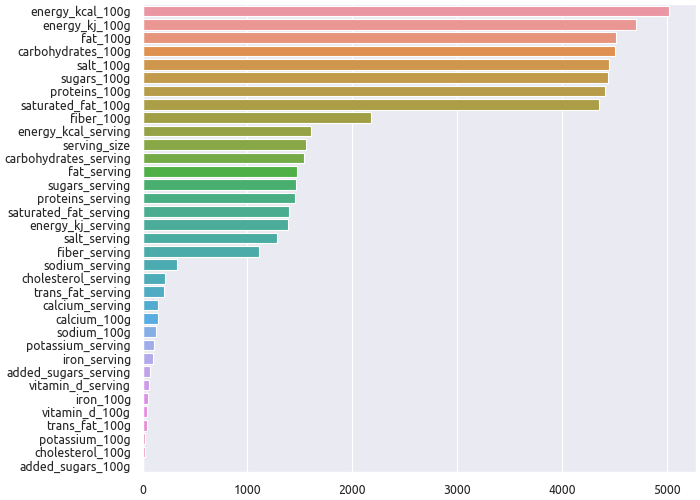
\includegraphics[width=8cm]{label_count}
	\caption{Number of occurrences of each entity class in the dataset}
	\label{fig:fig1}
\end{figure}

\subsection{Structure of the data}

The data consists of more than 3000 images that come with token-level annotations, exported as Parquet files. The dataset is split into a train set (2.88k images) and a test set (199 images).

Below is a description of the most important fields of the dataset:

\begin{itemize}
    \item \verb+tokens+: a list of tokens in the input image. This was extracted using Google Cloud Vision API.
    \item \verb+ner_tags+: a list of label IDs for each token in the input image. The label IDs are integers, and the mapping from label IDs to label names can be found in the Hugging Face dataset metadata. It is automatically available when loading the dataset using the \verb+dataset+ library.
    \item \verb+bboxes+: a list of bounding boxes for each token in the input image. The bounding boxes are in the format [\verb+x_min+, \verb+y_min+, \verb+x_max+, \verb+y_max+], where (\verb+x_min+, \verb+y_min+) is the top-left corner and (\verb+x_max+, \verb+y_max+) is the bottom-right corner of the bounding box. The bounding boxes are in the same order as the tokens. The coordinates should be normalized between 1 and 1000 (excluded). This was extracted from Google Cloud Vision OCR result as well.
    \item \verb+image+: the raw JPEG image (binary).
    \item \verb+meta+: a struct containing metadata about the sample.
\end{itemize}

\subsection{Statistics}

Across the entire dataset, the number of annotations for each entity (by removing the \verb+B-+ and \verb+I-+ prefixes for the entity name) can be found in Figure \ref{fig:fig1}).

We also used Google Cloud Vision to detect the most common language on each image (Table \ref{tab:table}). French, English, and Spanish are the 3 most common languages, making 72\% of all samples. The language distribution here is similar to what we observe in the Open Food Facts database.

\section{Model training}

We fine-tuned a LayoutLMv3-large model on this dataset, and reached a f1-score of 0.96. The resulting model is available on Hugging Face \footnote{\url{https://huggingface.co/openfoodfacts/nutrition-extractor}}.

All the code used for annotation, dataset generation, and model training can be found at:
\begin{center}
	\url{https://github.com/openfoodfacts/openfoodfacts-ai/tree/develop/nutrisight}
\end{center}

\begin{table}
	\caption{Main detected languages in the dataset}
	\centering
	\begin{tabular}{lll}
		\toprule
		Lang     & Count     & Percent \\
		\midrule
		French & 1098  & 35.61     \\
        English & 485 & 21.34 \\
        Spanish & 485 & 15.73 \\
        German & 238 & 7.72 \\
        Dutch & 212 & 6.88 \\
        Italian & 86 & 2.79 \\
        Unknown & 85 & 2.76 \\
        Portuguese & 44 & 1.43 \\
        Polish & 31 & 1.01 \\
        Finnish & 21 & 0.68 \\
		\bottomrule
	\end{tabular}
	\label{tab:table}
\end{table}

\section{Funding}

The NutriSight project has indirectly received funding from the European Union’s Horizon Europe research and innovation action programme, via the DRG4FOOD – Open Call \#1 issued and executed under the DRG4FOOD project (Grant Agreement no. 101086523).

\bibliographystyle{unsrtnat}
\bibliography{references}

\end{document}
